%--------------------------------------------------------------------------------
% CONFIGURATION DU DOCUMENT
%--------------------------------------------------------------------------------

\documentclass[a4paper,12pt]{report}

\usepackage[french]{babel}
\usepackage[utf8]{inputenc}
\usepackage[T1]{fontenc}
\usepackage{mathptmx}
\usepackage[most]{tcolorbox}
\usepackage[a4paper, left=2.5cm, right=2.5cm, top=2.5cm, bottom=2.5cm]{geometry}
\usepackage{graphicx}
\usepackage{lipsum}
\usepackage{hyperref}
\usepackage{amsmath, amssymb}
\usepackage{array}
\usepackage{float}
\usepackage{tabularx}

\usepackage{pgfplots}
\usepackage{tikz} 
\usetikzlibrary{shapes.geometric, arrows, arrows.meta}

\pgfplotsset{
    /pgfplots/layers/Bowpark/.define layer set={
        axis background,axis grid,main,axis ticks,axis lines,axis tick labels,
        axis descriptions,axis foreground
    }{/pgfplots/layers/standard},
}


\setlength{\textfloatsep}{10pt}

\newcolumntype{Y}{>{\centering\arraybackslash}X}



\begin{document}





%--------------------------------------------------------------------------------
% PAGE DE GARDE
%--------------------------------------------------------------------------------

\begin{titlepage}
    \centering

    %----------------------------------
    % Informations sur l'université
    %----------------------------------

    {\large Faculté des Sciences et Ingénierie - Sorbonne Université}\\[0.3cm]
    {\large Master Informatique parcours ANDROIDE}\\[1cm]
    
\includegraphics[width=0.3\textwidth]{./images/logo_SU.png}\\[1.5cm]


    %----------------------------------
    % Informations sur le projet
    %----------------------------------

    \vspace{1.5cm}

    {\LARGE LRC - Logique et représentations des connaissances}\\[1cm]
    {\Large Rapport de projet}\\[2cm]
    \rule{\linewidth}{0.5mm} \\[1cm]
    {\Huge \textbf{Subsomptions en Prolog}} \\[0.4cm]
    \rule{\linewidth}{0.5mm} \\[2cm]
    

    %----------------------------------
    % Informations sur nous
    %----------------------------------

    \begin{flushleft}
        \textbf{Réalisé par :} \\[0.3cm]
        PINHO FERNANDES Enzo \\[0.2cm]
    \end{flushleft}
    

    %----------------------------------
    % Date
    %----------------------------------

    \vfill
    {\large Décembre 2024}\\
    
\end{titlepage}





%--------------------------------------------------------------------------------
% Table des matières
%--------------------------------------------------------------------------------

\tableofcontents





%--------------------------------------------------------------------------------
% Pages d'introduction
%--------------------------------------------------------------------------------

\newpage

\chapter*{Introduction}
\addcontentsline{toc}{chapter}{Introduction}

Le but de ce projet est de programmer en Prolog un algorithme permettant d'inférer des subsomptions pour la logique de description \(FL^-\) décrite à la fin du sujet.
    On procède de façon progressive en ajoutant des règles pour gérer des cas de plus en plus complexes. On s'assure toujours de faire des inférences correctes : si on trouve
    que \(C\) subsume \(D\) selon nos règles, on a la garantie que \(C\) subsume bien \(D\). L'inverse n'est pas forcément vrai, le programme, construit progressivement, pouvant
    être incomplet.\\

Le rendu du projet doit comporter deux fichiers :
\begin{itemize}
    \item un fichier prolog, comportant en première ligne, en commentaire, les prénoms et noms des deux membres du binôme,
    \item un fichier pdf, comportant également en première ligne les prénoms et noms des deux membres du binôme et donnant les réponses aux questions de commentaire et logique.
\end{itemize}

\newpage





%--------------------------------------------------------------------------------
% Représentation
%--------------------------------------------------------------------------------

\newpage

\chapter*{Représentation}
\addcontentsline{toc}{chapter}{Représentation}





%--------------------------------------------------------------------------------
% Exercice 1
%--------------------------------------------------------------------------------

\section*{Exercice 1 : Représentation préfixe en prolog}
\addcontentsline{toc}{section}{Représentation préfixe en prolog}

On traduit les différents opérateurs de concepts et éléments des T-Box et A-Box de la façon suivante :
\begin{center}
    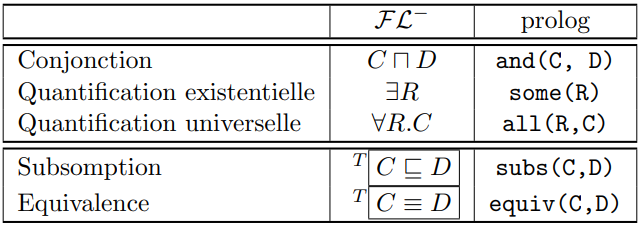
\includegraphics[width=0.6\textwidth]{./images/traduction_op.png}\\[1.5cm]
\end{center}

On travaille sur la T-Box correspondant aux connaissances sur les animaux suivant :
\begin{center}
    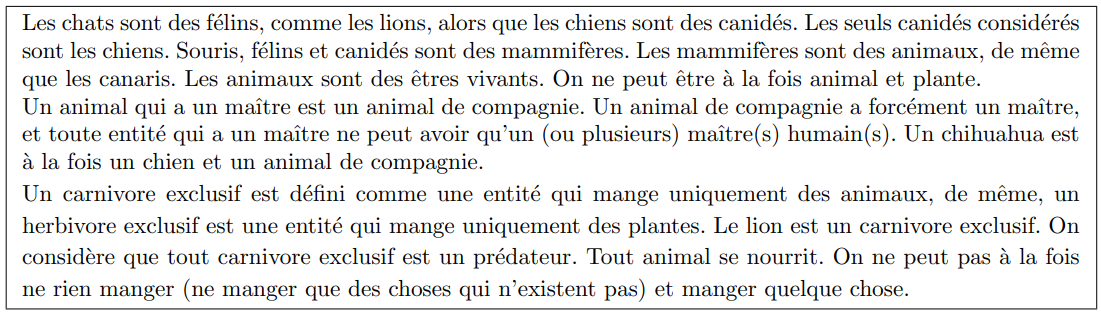
\includegraphics[width=1\textwidth]{./images/description_animaux.png}\\[1.5cm]
\end{center}

La traduction de ces connaissances en prolog est donnée dans le fichier \href{./src/LRC\_donneesProjet.pl}{LRC\_donneesProjet.pl}.
    Ouvrir ce fichier pour inspecter les données. Traduire en formules de \(FL^-\) les 6 lignes associées à l'indication \textbf{/* à commenter */} et
    identifier les phrases qu'elles traduisent.\\
    Note : \(\bot\) n'existant pas en \(FL^-\), on traite ici \textbf{nothing} comme un concept atomique.



\newpage

\begin{tcolorbox}[colback=gray!10, colframe=blue!30, coltitle=black, title=Réponse à l'exercice 1 - 1/1]

    Voici la traduction en \(FL^-\) des 6 lignes à commenter du fichier \href{./src/LRC\_donneesProjet.pl}{LRC\_donneesProjet.pl} ainsi que l'identification
        des phrases qu'elles traduisent dans la description des animaux vu précédemment.

    \begin{table}[H]
        \centering
        \setlength{\tabcolsep}{10pt}
        \begin{tabularx}{\textwidth}{|Y|}

            \hline \\[-0.4cm]
            \textbf{Code prolog} \\[0.3cm]
            \textbf{Traduction \(FL^-\)} \\[0.3cm]
            \textbf{Identification de la phrase} \\[0.1cm]
            \hline

            \hline \\[-0.4cm]
            \texttt{subs(chat,felin).} \\[0.3cm]
            \(chat \sqsubseteq felin\) \\[0.3cm]
            "Les chats sont des félins" \\[0.1cm]
            \hline

            \hline \\[-0.4cm]
            \texttt{subs(chihuahua,and(chien,pet)).} \\[0.3cm]
            \(chihuahua \sqsubseteq (chien \sqcap pet) \) \\[0.3cm]
            "Un chihuahua est à la fois un chien et un animal de compagnie." \\[0.1cm]
            \hline

            \hline \\[-0.4cm]
            \texttt{subs(and(animal,some(aMaitre)),pet).} \\[0.3cm]
            \((animal \sqcap \exists aMaitre) \sqsubseteq pet\) \\[0.3cm]
            "Un animal qui a un maître est un animal de compagnie." \\[0.1cm]
            \hline

            \hline \\[-0.4cm]
            \texttt{subs(some(aMaitre),all(aMaitre,personne)).} \\[0.3cm]
            \(\exists aMaitre \sqsubseteq \forall aMaitre.personne\) \\[0.3cm]
            "Toute entité qui a un maître ne peut avoir qu'un (ou plusieurs) maître(s) humain(s)." \\[0.1cm]
            \hline

            \hline \\[-0.4cm]
            \texttt{subs(and(all(mange,nothing),some(mange)),nothing).} \\[0.3cm]
            \((\forall mange.nothing \sqcap \exists mange) \sqsubseteq nothing\) \\[0.3cm]
            "On ne peut pas à la fois ne rien manger (ne manger que des choses qui n'existent pas) et manger quelque chose." \\[0.1cm]
            \hline

            \hline \\[-0.4cm]
            \texttt{equiv(carnivoreExc,all(mange,animal)).} \\[0.3cm]
            \(carnivoreExc \equiv \forall mange.animal\) \\[0.3cm]
            "Un carnivore exclusif est défini comme une entité qui mange uniquement des animaux." \\[0.1cm]
            \hline
            
        \end{tabularx}
    \end{table}

\end{tcolorbox}





%--------------------------------------------------------------------------------
% Subsomption structurelle pour FL-
%--------------------------------------------------------------------------------

\newpage

\chapter*{Subsomption structurelle pour \(FL^-\)}
\addcontentsline{toc}{chapter}{Subsomption structurelle pour \(FL^-\)}

Le but de cette section est d'écrire un ensemble de règles permettant de répondre à des questions du type "est-ce qu'on peut prouver que \(C\) est
    subsumé par \(D\) ?" (soit "est-ce que \(C \sqsubseteq_s D ?\)")\\

Il faut souligner la différentre entre \(\sqsubseteq\), qui correspond à des axiomes d'inclusion fournis explicitement dans la TBox, et \(\sqsubseteq_s\),
    qui correspond à des subsomptions que l'on peut prouver, à partir des axiomes fournis dans la TBox.





%--------------------------------------------------------------------------------
% Exercice 2
%--------------------------------------------------------------------------------

\section*{Exercice 2 : Concepts atomiques}
\addcontentsline{toc}{section}{Concepts atomiques}

On suppose que dans un premier temps que la TBox ne contient que des expressions du type \(A \sqsubseteq B\) où \(A\) et \(B\) sont des concepts
    atomiques et que \(C\) et \(D\) sont aussi atomiques. Pour vérifier si \(C \sqsubseteq_s D\) dans ce contexte, on propose les règles suivantes,
    à écrire dans votre fichier prolog, dans lequel vous aurez préalablement copié-collé le contenu du fichier \href{./src/LRC\_donneesProjet.pl}{LRC\_donneesProjet.pl}.\\\\
\texttt{subsS1(C,C).}\\
\texttt{subsS1(C,D) : -subs(C,D), C\textbackslash==D.}\\
\texttt{subsS1(C,D) : -subs(C,E), subsS1(E,D).}\\



%--------------------------------------------------------------------------------
% Question 2.1
%--------------------------------------------------------------------------------

\vspace{0.5cm}

\phantomsection
\addcontentsline{toc}{subsection}{1. Traduction des règles et tests}

\textbf{2.1)} Que traduisent ces règles ? Les tester sur les requêtes \(canari \sqsubseteq_s animal\), \(chat \sqsubseteq_s etreVivant\).



\begin{tcolorbox}[colback=gray!10, colframe=blue!30, coltitle=black, title=Réponse à la question 2.1 - 1/1]

    \textbf{Traduction des règles :}\\[-0.4cm]
    \begin{itemize}
        \item \texttt{subsS1(C,C)} : 
        \begin{itemize}
            \item Un concept est toujours subsumé par lui-même, on a donc \(C \sqsubseteq_s C\).
        \end{itemize}
        \vspace{0.3cm}

        \item \texttt{subsS1(C,D) :- subs(C,D), C\textbackslash==D} : 
        \begin{itemize}
            \item Si, dans la TBox, un concept \(C\) est subsumé par un concept \(D\) différent, alors on a \(C \sqsubseteq_s D\).
        \end{itemize}
        \vspace{0.3cm}

        \item \texttt{subsS1(C,D) :- subs(C,E), subsS1(E,D)} : 
        \begin{itemize}
            \item On peut y voir la règle de la transitivité. Si \(C \sqsubseteq E\), et \(E \sqsubseteq_s D\), alors on a \(C \sqsubseteq D\).
        \end{itemize}
    \end{itemize}

    \vspace{0.5cm}
    \hrule
    \vspace{0.5cm}

    Les requêtes renvoient true, ce qui est logique pour la première étant donné qu'on a bien \(canari \sqsubseteq animal\). Pour la deuxième, il existe une transition
        qui part de \(chat\) et qui arrive à \(etreVivant\), la voici : \((chat \sqsubseteq felin) \rightarrow (felin \sqsubseteq mammifere) \rightarrow (mammifere \sqsubseteq animal) 
        \rightarrow (animal \sqsubseteq etreVivant)\).  

\end{tcolorbox}



%--------------------------------------------------------------------------------
% Question 2.2
%--------------------------------------------------------------------------------

\newpage

\phantomsection
\addcontentsline{toc}{subsection}{2. Problème de la requête \(chien \sqsubseteq_s  souris\)}

\textbf{2.2)} Tester la requête \(chien \sqsubseteq_s  souris\). Quel problème pose cette requête ? Utiliser la trace pour en identifier la cause.



\begin{tcolorbox}[colback=gray!10, colframe=blue!30, coltitle=black, title=Réponse à la question 2.2 - 1/1]

    La requête \(chien \sqsubseteq_s  souris\) ne se termine jamais, dû à une boucle infinie au niveau de la règle de la transition. En effet, étant
        donné que \(chien\) et \(souris\) ne sont pas les mêmes concepts, et que nous avons pas \(chien \sqsubseteq souris\), alors le seul moyen est
        de trouver une transition de subsomption possible entre les deux.\\

    Pour cela, il essayera de commencer par la subsomption \(chien \sqsubseteq canide\) et cherchera donc à vérifier \(canide \sqsubseteq souris\). Même
        constat pour celui-ci. Il essayera plusieurs transitions qui rateront, jusqu'à qu'il fasse une transition \(canide \sqsubseteq chien\)... Et il
        cherchera à vérifier la requête initiale \(chien \sqsubseteq_s  souris\). Cela crée une boucle infinie.

    \vspace{0.5cm}
    \hrule
    \vspace{0.5cm}

    Voici l'exécution de la requête avec trace, et quelques commentaires dessus pointant le problème.
    \begin{center}
        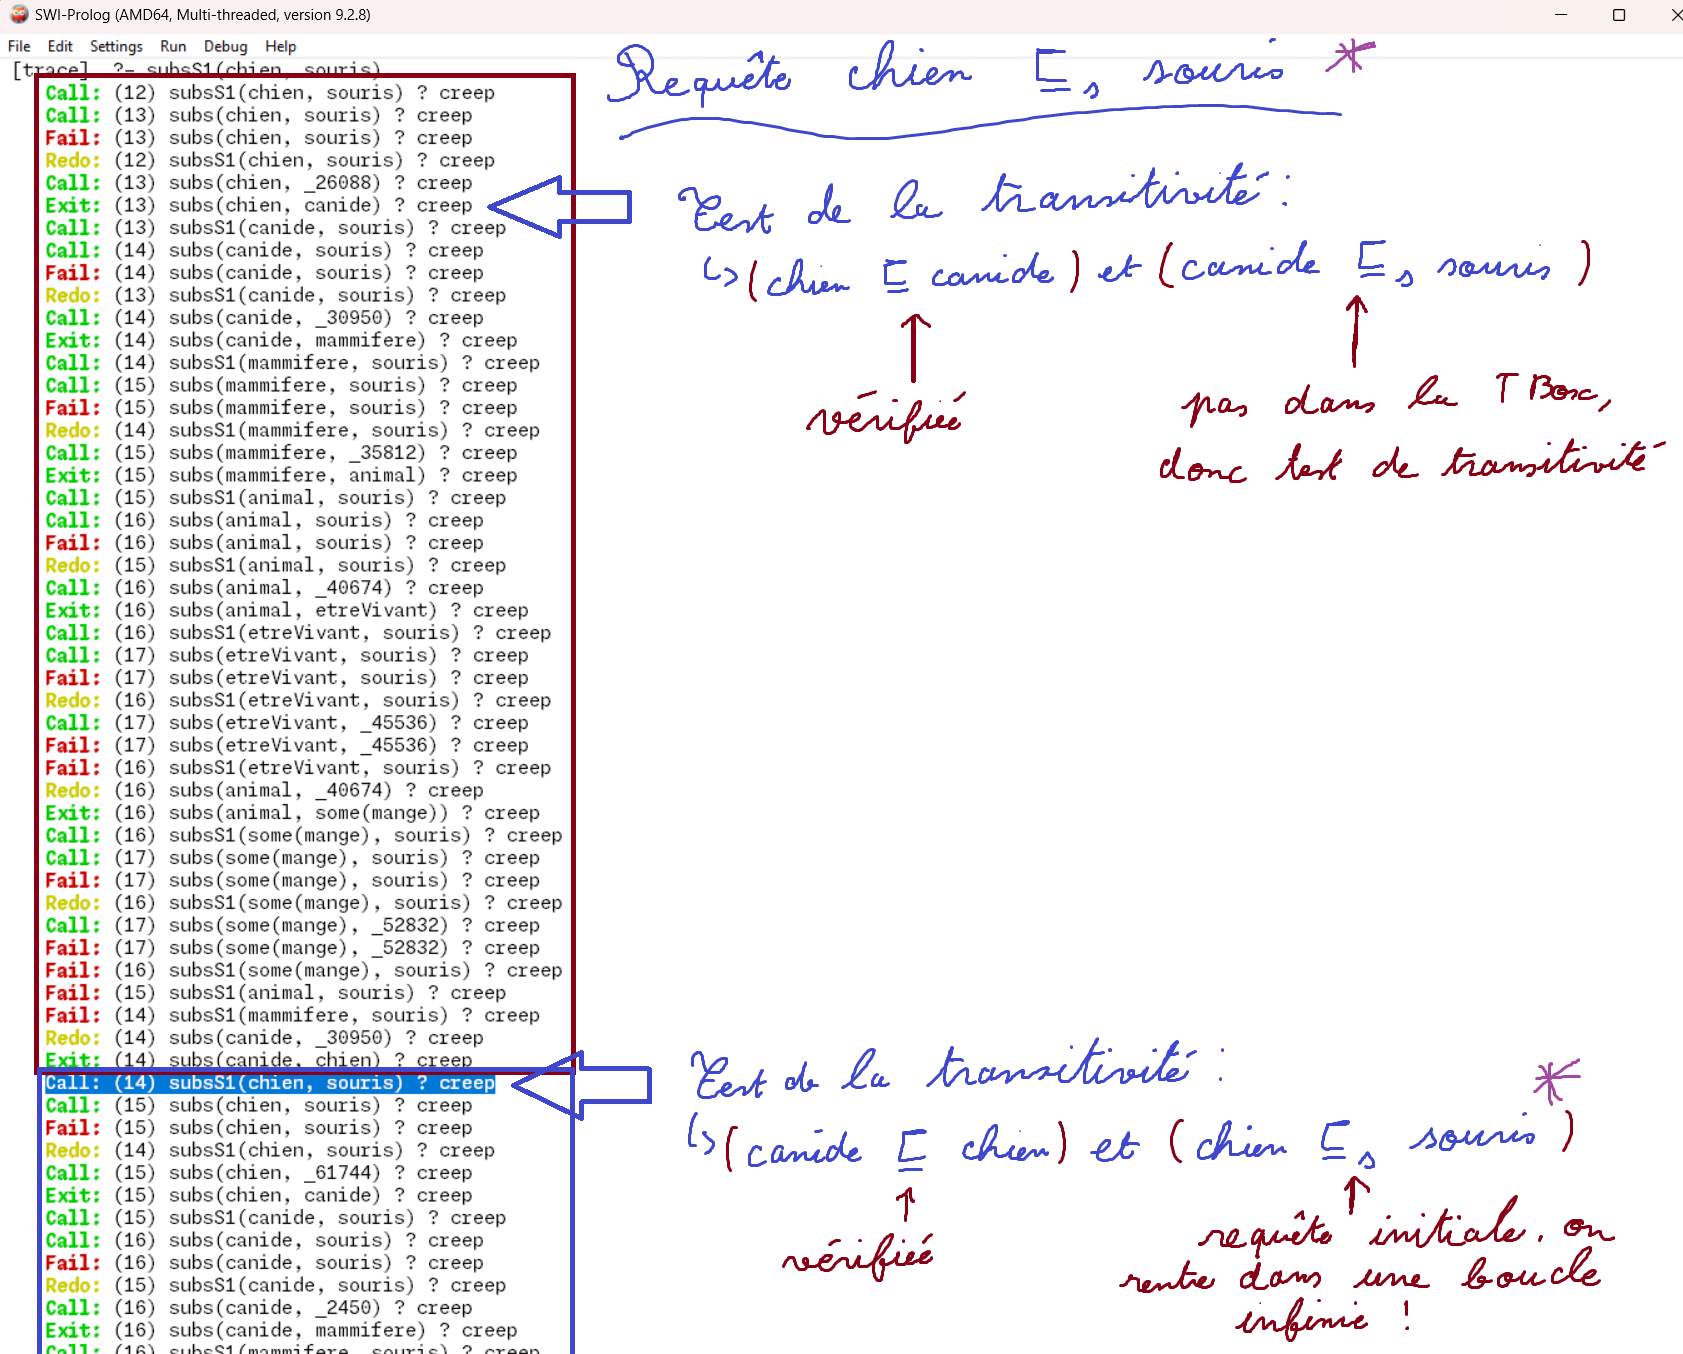
\includegraphics[width=1\textwidth]{./images/chien_souris_infini.png}\\[1.5cm]
    \end{center}


\end{tcolorbox}



%--------------------------------------------------------------------------------
% Question 2.3
%--------------------------------------------------------------------------------

\newpage

Pour corriger ce problème, on introduit un troisième argument contenant la liste des subsomptions déjà faites dans une branche. On définit \texttt{subsS(C,D)},
    qui doit être vérifié quand \(C \sqsubseteq_s D\), avec le prédicat auxiliaire \texttt{subsS(C,D,L)} où \(L\) contient la liste des concepts utilisés
    dans la preuve de la subsomption. Pour éviter des preuves infinies, on s'interdit de réutiliser un concept déjà présent dans \(L\).\\

On réécrit donc les règles sur \texttt{subsS1(C,D)} pour définir \texttt{subsS(C,D,L)}, en rajoutant avant tout appel récursif \(E \sqsubseteq_s D\)
    la condition que \(E\) ne soit pas dans \(L\) et en ajoutant \(E\) à \(L\) dans l'appel récursif :\\\\
\texttt{subsS(C,D) :- subsS(C,D,[C]).}\\
\texttt{subsS(C,C,\_).}\\
\texttt{subsS(C,D,\_) :- subs(C,D), C \textbackslash== D}\\
\texttt{subsS(C,D,L) : -subs(C,E), not(member(E,L)), subsS(E,D,[E|L]), E \textbackslash== D.}\\



\vspace{0.5cm}

\phantomsection
\addcontentsline{toc}{subsection}{3. Tests des nouvelles règles}



\textbf{2.3)} Tester ces nouvelles règles avec \(chat \sqsubseteq_s etreVivant\), \(chien \sqsubseteq_s canide\) et \(chien \sqsubseteq_s chien\) et
    vérifier que le résultat est conforme aux attentes. Tester ensuite la requête \(chien \sqsubseteq_s souris\) qui doit échouer. Inspecter la trace
    de cette requête.



\begin{tcolorbox}[colback=gray!10, colframe=blue!30, coltitle=black, title=Réponse à la question 2.3 - 1/1]

    Les requêtes \(chat \sqsubseteq_s etreVivant\), \(chien \sqsubseteq_s canide\) et \(chien \sqsubseteq_s chien\) renvoient tous true, ce qui est conforme
        à nos attentes. En ce qui concerne la requête \(chien \sqsubseteq_s souris\), elle échoue bien comme attendu. Avec la trace, nous pouvons constater
        qu'à chaque transition testée, on vérifie le contenu de la liste des concepts utilisés. Et celui-ci empêche bien la boucle infinie dû à la transition de
        \(canide\) et \(chien\).

    \vspace{0.5cm}
    \hrule
    \vspace{0.5cm}

    Voici l'exécution d'un bout de requête avec trace, sur la solution du problème de la boucle infinie.
    \begin{center}
        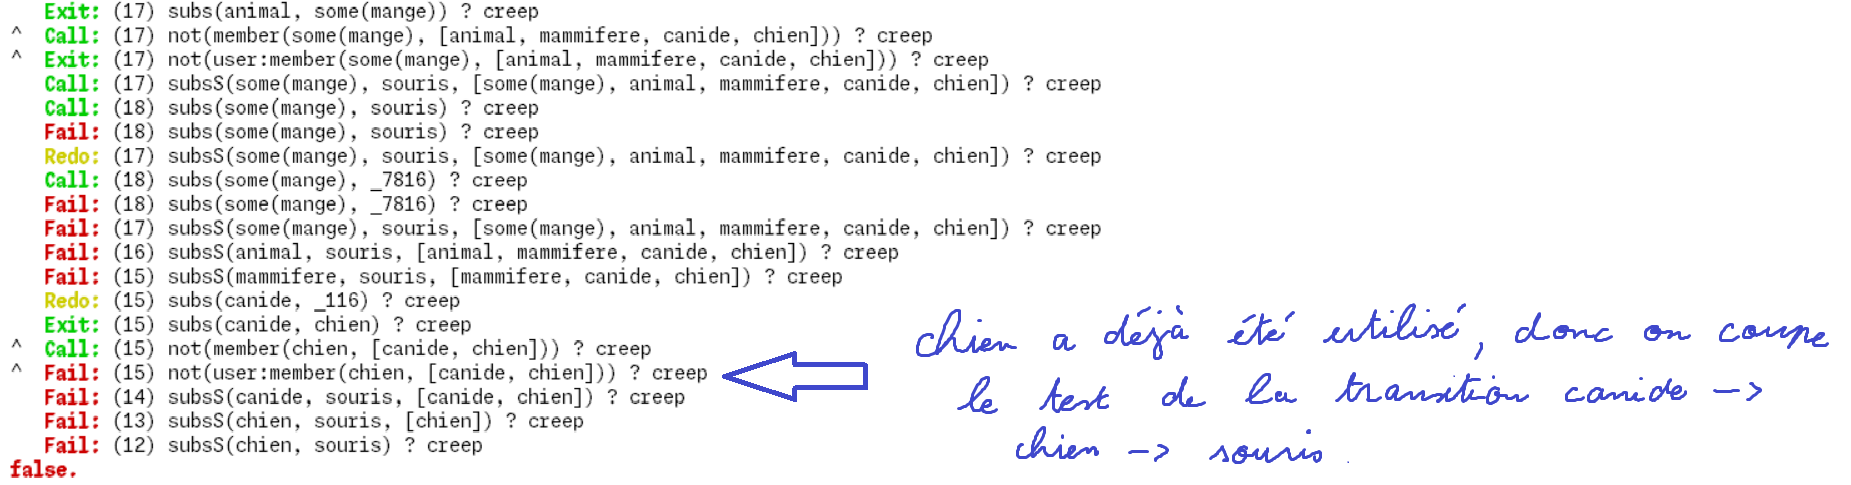
\includegraphics[width=1\textwidth]{./images/chien_souris_not_infini.png}\\[1.5cm]
    \end{center}

\end{tcolorbox}



%--------------------------------------------------------------------------------
% Question 2.4
%--------------------------------------------------------------------------------

\newpage

\phantomsection
\addcontentsline{toc}{subsection}{4. Test de la requête \(souris \sqsubseteq_s  \exists mange\)}

\textbf{2.4)} Tester la requête \(souris \sqsubseteq_s  \exists mange\). Pourquoi cette requête réussit-elle bien que \(\exists mange\) ne soit pas un concept atomique ?



\begin{tcolorbox}[colback=gray!10, colframe=blue!30, coltitle=black, title=Réponse à la question 2.4 - 1/1]

    Cette requête réussit bien que \(\exists mange\) n'est pas un concept atomique parce qu'il existe techniquement une transition de \(souris\) à \(some(mange)\)
        d'après notre TBox sur prolog. Ce dernier ne fait pas de "distinction" entre concept atomique et autre, et il trouve bien une valeur égale à \(some(mange)\).

    \vspace{0.5cm}
    \hrule
    \vspace{0.5cm}
        
    En effet, on peut suivre les étapes suivantes :\\[-0.4cm]
    \begin{itemize}
        \item \texttt{subsS(souris, some(mange)) :- subs(souris, mammifere), subsS(mammifere, some(mange))}\\[-0.2cm]
        \item \texttt{subs(souris, mammifere)} est vérifiée.
        \item \texttt{subsS(mammifere, some(mange)) :- subs(mammifere, animal), subsS(animal, some(mange))}\\[-0.2cm]
        \item \texttt{subs(mammifere, animal)} est vérifiée.
        \item \texttt{subsS(animal, some(mange))} est vérifiée grâce à la troisième règle, on trouve bien \texttt{subs(animal, some(mange))}.
    \end{itemize}

\end{tcolorbox}



%--------------------------------------------------------------------------------
% Question 2.5
%--------------------------------------------------------------------------------

\newpage

\phantomsection
\addcontentsline{toc}{subsection}{5. Requêtes \(chat \sqsubseteq_s X\) et \(X \sqsubseteq_s mammifere\)}

\textbf{2.5)} Que devraient renvoyer les requêtes \(chat \sqsubseteq_s X\) et \(X \sqsubseteq_s mammifere\) ? Vérifier que c'est bien le cas (il n'est pas nécessaire
    d'éliminer les réponses doubles ou le false final).



\begin{tcolorbox}[colback=gray!10, colframe=blue!30, coltitle=black, title=Réponse à la question 2.5 - 1/1]

    La requête \(chat \sqsubseteq_s X\) est sensée renvoyer "tout ce qu'un chat puisse être" par la variable X d'après notre TBox. Dans ce cas là, nous devrions avoir plusieurs
        résultats pour X. Un chat est un \textbf{chat} (subsumé par lui-même), un \textbf{félin}, un \textbf{mammifere}, un \textbf{animal}, un \textbf{être vivant} et
        pour la même raison qu'à la question 2.4, il devrait renvoyer \textbf{some(mange)}, parce qu'un animal mange toujours au moins une chose et que prolog le renvoie.\\

    \vspace{0.5cm}
    \hrule
    \vspace{0.5cm}
          
    La requête \(X \sqsubseteq_s mammifere\) est sensée renvoyer "toute entité étant un mammifere", dans notre TBox, les \textbf{félins, canidés et souris} seront renvoyés, ainsi 
        que \textbf{mammifère} parce que tout concept est subsumé par lui-même. Bien évidemment, on aura aussi les \textbf{chiens, chats et lions} qui seront renvoyés, parce qu'ils
        sont subsumés par \texttt{felin} et \texttt{canide}.

    \vspace{0.5cm}
    \hrule
    \vspace{0.5cm}

    Voici la vérification de notre réponse sur prolog, on a bien les mêmes résultats, ainsi qu'un false final, parce que Prolog teste d'autres possibilités même après avoir trouvé
        toutes les solutions réalisables.\\[0.5cm]
    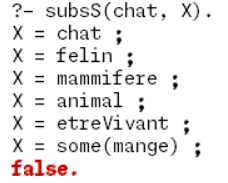
\includegraphics[width=0.5\textwidth]{./images/chat_X.png}
    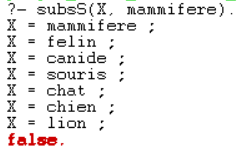
\includegraphics[width=0.5\textwidth]{./images/X_mammifere.png}

\end{tcolorbox}



%--------------------------------------------------------------------------------
% Question 2.6
%--------------------------------------------------------------------------------

\newpage

\phantomsection
\addcontentsline{toc}{subsection}{5. Règles pour l'équivalence, et requête \(lion \sqsubseteq_s \forall mange.animal\)}

\textbf{2.6)} Ecrire des règles permettant de dériver \(A \sqsubseteq B\) et \(B \sqsubseteq A\) à partir de \(A \equiv B\). Tester avant et 
    après ajout des règles la requête \(lion \sqsubseteq_s \forall mange.animal\).



\begin{tcolorbox}[colback=gray!10, colframe=blue!30, coltitle=black, title=Réponse à la question 2.6 - 1/1]

    Pour commencer, testons la requête avant l'ajout des règles. Prolog nous renvoie tout simplement \textbf{false}. En effet, nous avons aucune
        subsomption dans la TBox de type \(subs(X, all(mange, animal))\), \(X\) étant une variable. On ne peut donc pas trouver de transition, et 
        on ne peut pas utiliser l'équivalence \(carnivoreExc \equiv \forall mange.animal\) dû à l'absence des règles.

    \vspace{0.5cm}
    \hrule
    \vspace{0.5cm}

    Afin d'ajouter les règles, il faut savoir que \(C \equiv D \Rightarrow (C \sqsubseteq D) \land (D \sqsubseteq C)\). Il suffit donc de rajouter
        deux nouvelles règles cherchant si \(C \equiv D\) est dans la TBox, pour \(C \sqsubseteq D\) et \(D \sqsubseteq C\) séparémment. On a donc :\\\\
    \texttt{subs(C, D) :- equiv(C, D).}\\
    \texttt{subs(D, C) :- equiv(C, D).}\\

    L'ajout se trouve aux lignes 61-63 du fichier \href{./src/LRC\_donneesProjet.pl}{LRC\_donneesProjet.pl}.

    \vspace{0.5cm}
    \hrule
    \vspace{0.5cm}

    Avec les nouvelles règles, prolog nous renvoie \textbf{true}. En effet, il va en premier lieu tester plusieurs transitions de subsomption jusqu'à tomber
        sur celle allant de \(lion\) à \(carnivoreExc\). Ensuite, il essayera donc de prouver que \(subsS(carnivoreExc, all(mange, animal))\) ce qu'il y arrivera
        grâce à l'équivalence \(equiv(carnivoreExc, all(mange, animal))\).\\

    Ensuite, il cherchera toujours d'autres chemins possible, sans résultat, renvoyant un false.

\end{tcolorbox}





\end{document}